In this section, the multi-modality strategy will be experimented on synthetic dictionaries and real EEG/MEG lead-fields.
In all of the experiments, the agglomerative hierarchical clustering analysis based on the block structure identification framework proposed in Chapter \ref{sec:Clustering} will be applied on the dictionaries.

The proposed inter-block coherence measure in a special case, Block-MCC$_{2,2}$\footnote{\emph{$({2,2})$-Block Mutual Coherence Constant}}, is used to compute the similarity matrix in the hierarchical clustering algorithm, i.e., $M_{2,2}(\myPhi) \seq \max_{k,k' \neq k} \Vert \myPhi^\dagger[k] \myPhi [k'] \Vert_{2 {\to} 2} /d_{max} $.
%The $M_{1,\infty}(\myPhi)$ is selected, because the fraction $\Vert \boldsymbol{x} \Vert_{\boldsymbol{w};p,1} / \Vert \boldsymbol{x} \Vert_{\boldsymbol{w};q,1}$ in Corollary \ref{crl:BERC-BMIC} is maximized for $q \seq 1$ and $p \seq \infty$.
%\begin{equation*}
%M_{1,\infty}\myparanthese{\myPhi} 
%= \max_{k,k' \neq k} \frac{d_{k'}}{d_{max}} \mynorm{\myPhi^\dagger\mybracket{k} \myPhi \mybracket{k'}}_{1,\infty}.
%\end{equation*}
\myhl{The standard complete method is used to compute the inter-cluster distance required in the hierarchical clustering algorithm.}
%------------------------------------------------------
\subsection{Synthetic dictionary}
In this part, the set of two complementary random dictionaries $\myPhi_i \ssin \mathbb{R}^{10 \stimes 80}$, $i \seq \{\boldsymbol{1} , \boldsymbol{2} \}$, with equally-sized blocks of length $d_j \seq d \seq 2$, $\forall j$, is generated from independent and identically distributed (i.i.d.) random variables and all columns of the dictionaries are normalized to have unit $\ell_2$ norm.

%In this chapter, the experiments of multi-modality have done on synthetic dictionaries and real EEG/MEG leadfields.
%In the experiment with synthetic data, 
In order to generate two complementary random dictionaries, 
%and to ultimately combine them, 
firstly, as described in Section \ref{sec:Artificial simulated dictionary}, one of the dictionaries is generated by setting the related parameters $\varepsilon_{inter}$ and $\varepsilon_{intra}$.
Then, utilising the same strategy and by setting the parameter $\varepsilon_{inter-dictionary}$, which controls the overlap between the two dictionaries, the second dictionary is produced.
In figure \ref{fig:Multomodal-Phi}(a) and (b), the role of different types of $\varepsilon$ in generation of random dictionaries $\myPhi_{\boldsymbol{1}}$ and $\myPhi_{\boldsymbol{2}}$ is shown.
Then, as shown in figure \ref{fig:Multomodal-Phi}(c) by drawing half of the rows of each of the dictionaries and finally by making a sufficient shift on one of the set of rows belonging to one dictionary, here $\myPhi_{\boldsymbol{2}}$, the combined dictionary $\myPhi_{\boldsymbol{12}}$ is obtained.
All the results are shown in average and standard deviation over 100 repetitions of generation of complementary random dictionaries pairs.
\begin{figure}[!b]
\centering
\includegraphics[width=1\textwidth,keepaspectratio]{images/Multomodal-Phi.png} % width=0.5\textwidth  scale=0.49
\centering
\caption{The role of (a) $\varepsilon_{inter}$ and $\varepsilon_{intra}$ in generation of random dictionary $\myPhi_{\boldsymbol{1}}$, and (b) $\varepsilon_{inter-dictionary}$ in generation of $\myPhi_{\boldsymbol{2}}$ to produce the multi-modal dictionary $\myPhi_{\boldsymbol{12}}$.}
\label{fig:Multomodal-Phi}
\end{figure}
\FloatBarrier
%\newpage
%------------------------------------------------------
\paragraph{Block-ERC in clustered representation for a combined dictionary}
%\subsubsection{Effect of clustering the coherent blocks of a combined dictionary on Block-ERC based on Block-MCC$_{q,p}$} \footnote{\emph{Block-sparse Exact Recovery Condition(s)}} \footnote{\emph{Block-sparse Exact Recovery Condition(s)}}
In Section \ref{sec:clusteringOFcoherent_BERC-BMIC}, we demonstrated that in a random dictionary with certain values of $\varepsilon_{inter}$ and $\varepsilon_{intra}$, the $\myBSLTxt_{2,2}$\footnote{\emph{$(2,2)$-Block-Sparsity Level}} computed in each clustering level of the hierarchical clustering algorithm have a peak value at a clustering level equal to the number of clusters in the generated dictionary.

Therefore, under certain values of $\varepsilon_{inter}$ and $\varepsilon_{intra}$, the argument of the peak in $\myBSL_{2,2}(\myPhi)[\%]$ computed at each level of the hierarchical clustering algorithm is equal to the number of clusters in the dictionary, i.e., $N$.

In this part, in an experiment similar to Section \ref{sec:clusteringOFcoherent_BERC-BMIC}, the block sparsity-level in the pessimistic case, i.e., $\myBSL_{2,2}(\myPhi)[\%]$, is computed in each clustering level of the 
hierarchical clustering analysis, but here the dictionary 
%instead of being a simple random matrix 
is a combination of two complementary dictionaries instead of being a simple mono-modal random matrix.
In Section \ref{sec:Multimodal Structure and the model}, the procedure of combining two complementary dictionaries is described.
Also, the complementarity of two dictionaries is defined based on their overlap, determined by $\varepsilon_{inter-dictionary}$.

In generating two complementary dictionaries, one of them is produced as explained in Section \ref{sec:Artificial simulated dictionary}. 
Then the other dictionary is generated by multiplying the first dictionary to a random matrix $\exp((\boldsymbol{C} \sm \boldsymbol{C}^T) \sqrt{2} \varepsilon_{inter-dictionary} / \Vert \boldsymbol{C} \sm \boldsymbol{C}^T \Vert_F)$, where, $\boldsymbol{C}$ is a square random matrix of dimension $m$.

As it can be seen in figure \ref{fig:SL_Hierarchical_Multimodal}, by applying hierarchical clustering on the blocks of the combined dictionary for $\varepsilon_{inter-dictionary} \seq 1$, $\varepsilon_{inter} \sgeq 3.5$ and $\varepsilon_{intra} \sleq 0.1$, a peak in $\myBSL_{2,2}(\myPhi)[\%]$ appears in an argument equal to the sum of the clusters in each of the two original dictionaries.

For instance, when there are four clusters in each of the two complementary dictionaries i.e., $N \seq 4$ (blue squares), which construct the combined one, the maximum $\myBSL_{2,2}(\myPhi)[\%]$ for combined dictionary is at the eighth clustering level.

Similarly the consistent results are obtained for five clusters in each of the two complementary dictionaries, i.e., $N \seq 5$ (red circles).
In other words, there is a peak in $\myBSL_{2,2}(\myPhi)[\%]$ at the tenth clustering level, when the multi-modal dictionary is composed of two mono-modal dictionaries, each has five clusters.
For the clustering level lower than the optimal level, the space is under-sampled and there would be a block spanning the whole space, whereas for the clustering level higher than the optimal level, the space is over-sampled and the over-partitioning leads to high coherence measure.

On the other hand, when the average blocks of each cluster of blocks are not different enough, i.e., $\varepsilon_{inter} \sless 3.5$, but still the blocks in each cluster of blocks are similar enough, i.e., $\varepsilon_{intra} \sleq 0.1$, we can observe that the number of clusters in the combined dictionary or the argument of the peak in $\myBSL_{2,2}(\myPhi)[\%]$ is less than the sum of clusters in each of initial dictionaries but greater than the number of clusters in each of initial dictionaries.
\newpage

Therefore, the number of clusters in the combined dictionary depending on the overlap between the blocks, which is determined by $\varepsilon$, is greater than the number of clusters in one of the initial dictionaries and at most is equal to the sum of the number of clusters in the initial dictionaries.

In addition, the amplitude of peak of $\myBSL_{2,2}(\myPhi)[\%]$ increases when the number of clusters decreases.
For instance, in figure \ref{fig:SL_Hierarchical_Multimodal}, the amplitude of average peak of $\myBSL_{2,2}(\myPhi)[\%]$ for multi-modal dictionaries composed of two four-clusters dictionaries (blue square) is higher than the corresponding average amplitude for five clusters in each of mono-modal dictionaries (red circle).

Therefore, by reducing the number of clusters in the dictionary, $\myBSL_{2,2}(\myPhi)[\%]$ increases, hence, more weakened Block-ERC\footnote{\emph{Block-sparse Exact Recovery Condition(s)}} are obtained. 
%As it can be seen in figure \ref{fig:SL_Hierarchical_Multimodal}, the average peak of the multi-modal dictionaries with eight clusters (blue squares) is higher than the average peak of the multi-modal dictionaries with ten clusters (red circles)
\begin{figure}[!b]
\centering
\includegraphics[width=1\textwidth,keepaspectratio]{images/SL_Hierarchical_Multimodal.png} % width=0.5\textwidth  scale=0.49
\centering
\caption{$\myBSL_{2,2}(\myPhi)[\%]$ for each level of clustering is computed for the complete method, Block-MCC$_{2,2}$, $d \seq 2$, $N \seq \{4 , 5 \}$, $\varepsilon_{inter-dictionary} \seq 1$, and different values of $\varepsilon_{inter}$ and $\varepsilon_{intra}$ for simulating dictionary $\myPhi \ssin \mathbb{R}^{10 \stimes 80}$.}
\label{fig:SL_Hierarchical_Multimodal}
\end{figure}
\FloatBarrier
%------------------------------------------------------
\subsection{Real EEG and MEG lead-field}
In this part, the original lead-fields, which build the multi-modal lead-field are the ones explained in Section \ref{sec:Real EEG/MEG leadfield}.
Therefore, there are three head models with spherical, realistic inflated, and realistic highly-folded cortical sheets as shown in figure \ref{fig:Sensor_vol_Source_EMEG}.

The 32 sensors shown in figure \ref{fig:Sensor_vol_Source_EMEG} are in multi-modal case, where, there are equal number of sensors from both modalities.
By selecting the odd and even rows of EEG and MEG USLE, respectively, we can see that the sensor distribution is almost uniform, i.e., the sensors are not concentrated in a region of brain.
\begin{figure}[!b]
\centering
\includegraphics[width=1\textwidth,keepaspectratio]{images/Sensor_vol_Source_EMEG.png} % width=0.5\textwidth  scale=0.49
\centering
\caption{(a) spherical, (b) realistic inflated and (c) realistic highly-folded cortical sheets for the head models used in EEG and MEG multi-modality experiment.}
\label{fig:Sensor_vol_Source_EMEG}
\end{figure}
%\FloatBarrier
%------------------------------------------------------
\paragraph{EEG and MEG complementarity in brain source segmentation}
In Section \ref{sec:EMEG_Complementarities}, some basic complementarities of EEG and MEG were discussed.
In this section we show that in the brain source segmentation using the proposed strategy of clustering coherent lead-fields corresponding to brain sources utilising Block-MCC$_{q,p}$, we can observe some complementarities between brain source segmentation employing EEG or MEG lead-field.

In figure \ref{fig:EMEG_complementarities}, the brain clusters or regions based on clustering of the EEG or MEG lead-field for clustering levels 3, 10, 15, 17, and 20 and three types of cortical sheets are shown.

It can be seen that for the all shown clustering levels, the previously mentioned complementarity also appears in our brain source segmentation strategy, which is more visible in low clustering levels in figure \ref{fig:EMEG_complementarities}.
%For instance in figure \ref{fig:EMEG_complementarities}(a), for the brain source segmentation using EEG leadfield at the third clustering level, the occipito-parietal (left and right hemisphere in different segments) and frontal lobes are appeared whereas using MEG leadfield results in temporal brain lobes (see figure \ref{fig:Sensor_vol_Source_EMEG} for the orientation of head), which are complementary.
%In higher clustering levels, e.g., for 17 clusters, other than revealing some complementary precise regions, generally utilizing the EEG leadfield results in the segmentation of the left and right hemisphere while the MEG leadfield results in segmenting the central part as shown in figure \ref{fig:EMEG_complementarities}.
\begin{figure}[!b]
\centering
\includegraphics[width=0.9\textwidth,keepaspectratio]{images/EMEG_complementarities.png} % width=0.5\textwidth  scale=0.49
\centering
\caption{EEG and MEG complementarity in brain source segmentation using Block-MCC$_{2,2}$ and complete method for some clustering levels and for (a) spherical, (b) realistic inflated, and (c) realistic highly-folded cortical sheets.}
\label{fig:EMEG_complementarities}
\end{figure}
\FloatBarrier
%------------------------------------------------------
\paragraph{EEG and MEG multi-modality and the clustering tree}
\label{EEG and MEG multimodality and the clustering tree} 
The agglomerative hierarchical cluster analysis, using the standard inter-cluster distance and our proposed inter-block similarity methods builds a hierarchy of clustering structures, which is represented in the clustering tree, as shown in figure \ref{fig:EMEG_Multimodality_Dendrogram}.

The clustering trees built using EEG, MEG, and multi-modal EEG+MEG lead-fields for spherical, realistic inflated, and realistic highly-folded cortical sheets are shown in figure \ref{fig:EMEG_Multimodality_Dendrogram}(a), (b), and (c), respectively. 

As mentioned before, the advantage of using the hierarchical clustering algorithm is in estimating the number of clusters and in general the block structure, by selecting a block structure corresponding to the longest inter-node distance.
Also, one can impose other constraints such as minimum number of clusters.

In figure \ref{fig:EMEG_Multimodality_Dendrogram}, for each source model, the block structure is opted based on a minimum number of clusters and maximum inter-node distance.
To make clusters distinguishable, each cluster is colour-coded.
\begin{figure}[!b]
\centering
\includegraphics[width=0.8\textwidth,keepaspectratio]{images/EMEG_Multimodality_Dendrogram.png} % width=0.5\textwidth  scale=0.49
\centering
\caption{Clustering tree using EEG or MEG mono-modal lead-field and EEG+MEG multi-modal lead-field for (a) spherical, (b) realistic inflated, and (c) realistic highly-folded cortical sheets.}
\label{fig:EMEG_Multimodality_Dendrogram}
\end{figure}
\FloatBarrier
%------------------------------------------------------
\paragraph{EEG and MEG multi-modality and the number of regions}
\label{EEG and MEG multimodality and the number of regions}
%\subsubsection{EEG and MEG multimodality and the number of regions}
%In figure \ref{fig:EMEG_SL}, the maximum sparsity level in the most optimistic case is shown for the leadfields of EEG, MEG, and their combination computed for six tractable similarity measures BMIC and four algorithms calculating inter-clusters distance, named 'Average', 'Complete', 'Weighted', and 'Ward'.
%The leadfields are obtained using spherical volume conduction head model.
%As can be seen in figure \ref{fig:EMEG_SL}, in most cases the sparsity level resulted from the combination of EEG and MEG leadfields is higher than that of EEG or MEG leadfield alone.
%\begin{figure}[!b]
%\centering
%\includegraphics[width=1\textwidth,keepaspectratio]{images/EMEG_SL.png} % width=0.5\textwidth  scale=0.49
%\centering
%\caption{Maximum sparsity level in the most optimistic case for the leadfield of EEG, MEG, and their combination computed for six tractable similarity measures BMIC and four algorithms calculating inter-clusters distance, named 'Average', 'Complete', 'Weighted', and 'Ward'.}
%\label{fig:EMEG_SL}
%\end{figure}
In order to estimate the number of clusters from the dendrogram as described in Section \ref{sec:hierarchical_cluster_estim}, in addition to the constraint of the maximum distance between consecutive nodes or clusters in dendrogram, the number of clusters is also set to be greater than a threshold.

As it can be seen in figure \ref{fig:EMEG_Multimodality}(a), the estimated number of clusters or brain regions resulted from the EEG and MEG multi-modal lead-field for spherical cortical sheet is 10, which is more than the estimated number of brain regions using EEG or MEG lead-field alone, which both are 8 clusters. %, respectively.
The similar results are obtained for realistic head models as shown in figure \ref{fig:EMEG_Multimodality}(b) and (c).

Therefore, brain source space segmentation using the proposed strategy of clustering the coherent lead-fields based on the introduced Block-MCC$_{2,2}$ is more refined when utilising EEG and MEG multi-modal lead-field compared to EEG or MEG mono-modal lead-fields.
%by utilizing EEG and MEG multi-modal leadfield the brain segmentation will be more refined.
%In addition the maximum sparsity levels are higher than those in unimodal dataset, which means that multi-modality can improve the block-sparse exact recovery conditions through increasing the sparsity levels.
\begin{figure}[!b]
\centering
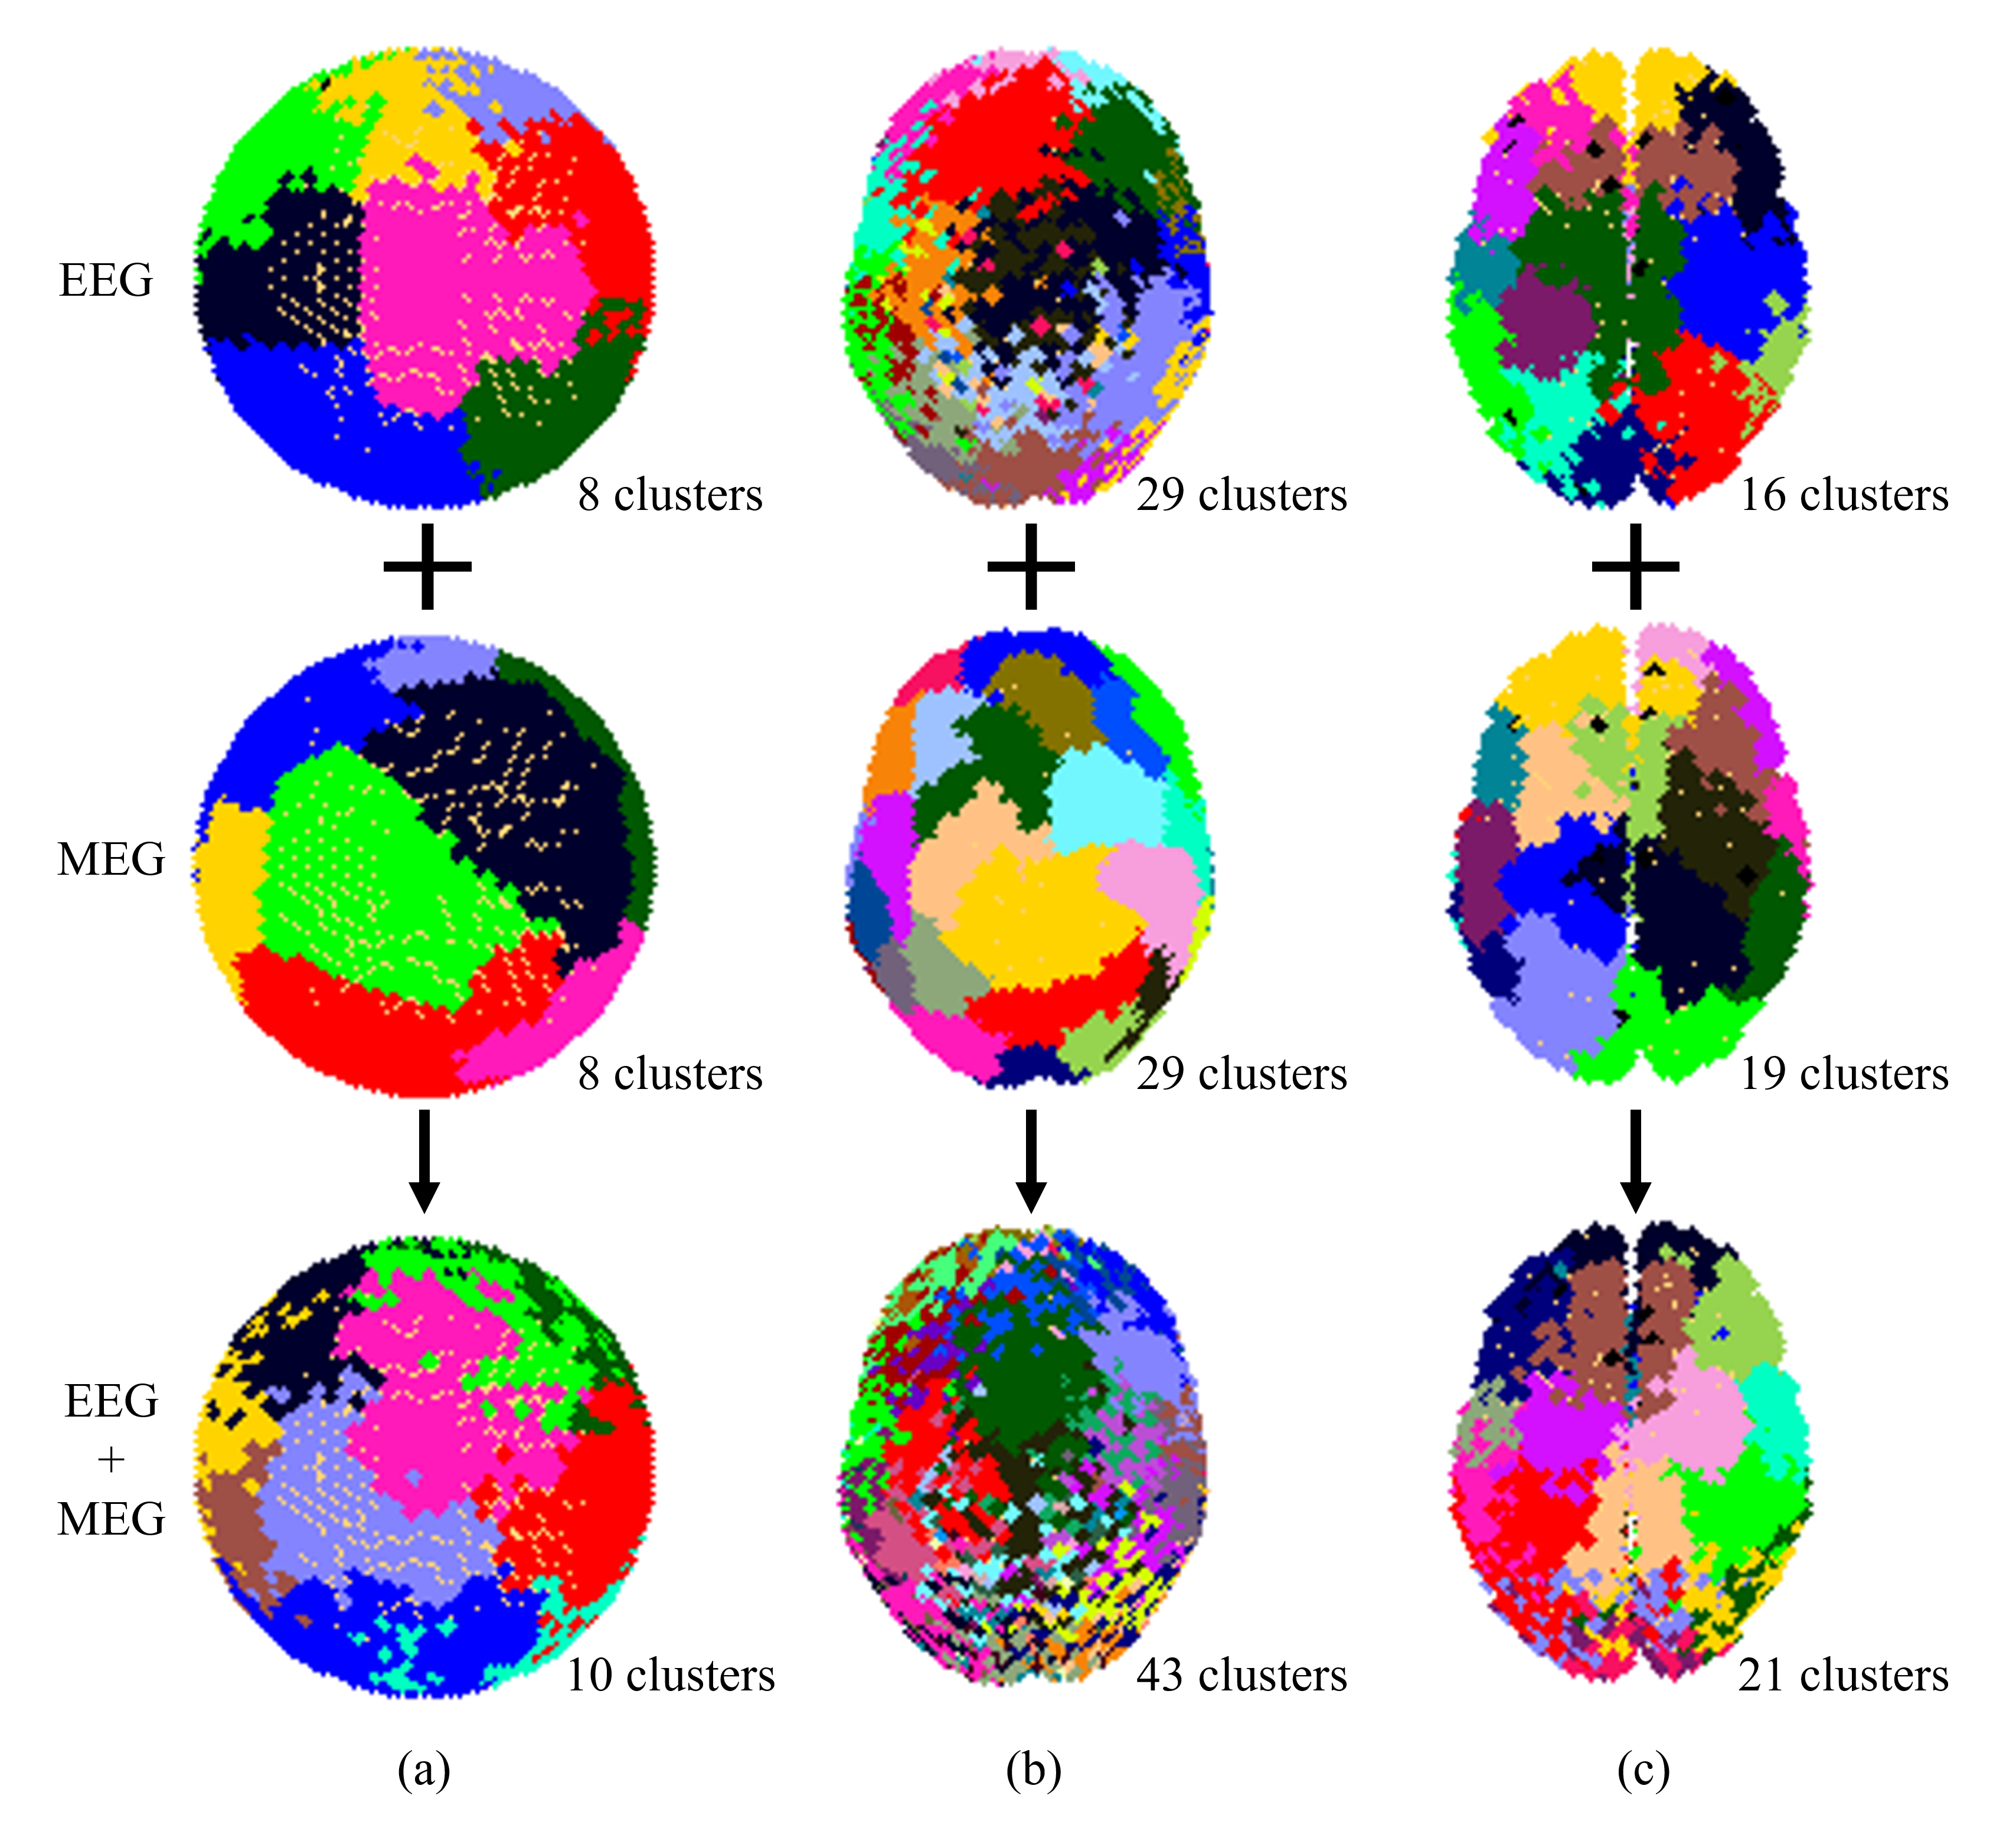
\includegraphics[width=0.8\textwidth,keepaspectratio]{images/EMEG_Multimodality.png} % width=0.5\textwidth  scale=0.49
\centering
\caption{Number of clusters using EEG or MEG mono-modal lead-field and EEG+MEG multi-modal lead-field for (a) spherical, (b) realistic inflated, and (c) realistic highly-folded cortical sheets.}
\label{fig:EMEG_Multimodality}
\end{figure}
\FloatBarrier
%------------------------------------------------------
\paragraph{EEG and MEG multi-modality and the area of regions}
In this part, for a fixed number of regions or clusters, the area of brain regions is investigated for EEG/MEG mono-modal lead-fields and multi-modal EEG and MEG lead-field clustering.

In this experiment, to better demonstrate the impact of multi-modality on the area of brain regions, only the source model with spherical cortical sheet is used.
In addition the standard \emph{average} method is used to compute the inter-cluster distance.
In this method, the distance between two clusters is defined as the average distance between each point in one cluster to every point in the other cluster.
Furthermore, the Block-MCC$_{1,\infty}$ is used as coherence measure.

In the top row of figure \ref{fig:EMEG_regionsArea}, it can be seen that in each certain number of clusters, the biggest area (maximum value in bar chart) belongs to multi-modal EEG and MEG lead-field clustering and nearly for all the other regions the area for multi-modal EEG and MEG is less than EEG or MEG lead-field alone. 

In addition, the area of brain regions are represented in pie charts.
The largest area is coloured as blue in pie charts, which is not very obvious in brain source space in the current angle of view.
Because, the region with maximum area represents brain sources at the bottom of the head, where, there is not any sensor on it, whereas the other regions represent brain sources under the sensors.
%For multi-modal EEG and MEG leadfield clustering, these values are lower than EEG or MEG

Therefore, for a fixed number of clusters, brain regions under sensors in multi-modal lead-field clustering are smaller than mono-modal lead-field clustering.
Hence, EEG and MEG multi-modality leads to increased brain source space resolution.
%the other advantage of multi-modality is increase in brain source space resolution.
\begin{figure}[!b]
\centering
\includegraphics[width=1\textwidth,keepaspectratio]{images/EMEG_regionsArea.png} % width=0.5\textwidth  scale=0.49
\centering
\caption{At each level of clustering, the area of brain regions are shown in pie and bar charts for EEG, MEG and their combination. At the top row, the descendingly sorted brain regions are shown for each one of three types of lead-fields. The hierarchical clustering method is average, and BMIC$_{1,\infty}$ is used as coherency measure.
}
\label{fig:EMEG_regionsArea}
\end{figure}
\FloatBarrier
